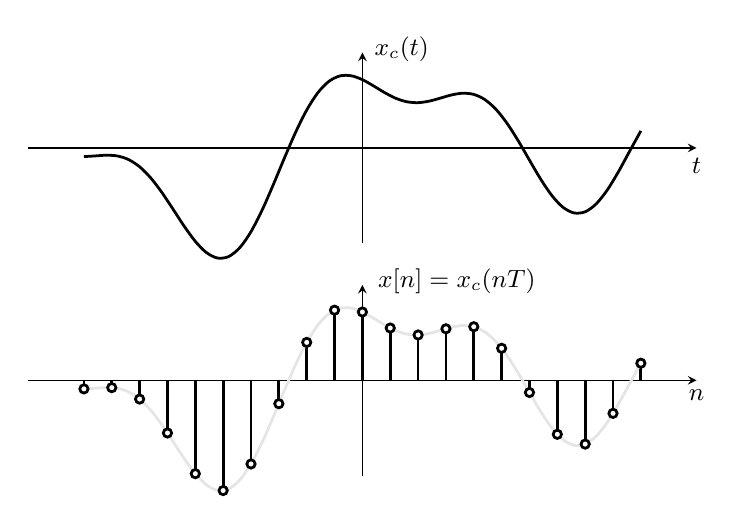
\begin{tikzpicture}
\begin{axis}[
	name=plot1,
	axis lines*=middle,
	enlargelimits = true,
	clip=false,
	scale only axis,
	width=0.7\textwidth,
	height=0.2\textwidth,
	ymin=-2.5,
	ymax=2.5,
	xmin=-10,
	xmax=10,
	axis line style={->,>=stealth},
	xlabel={\small $t$},
	ylabel={\small $x_c(t)$},
	every axis x label/.style={
		at={(ticklabel* cs:1)},
		%xshift=0.2cm,
		anchor=north,
	},
	every axis y label/.style={
		at={(ticklabel* cs:0.9)},
		anchor=south,
		xshift=0.5cm,
	},
	xtick=\empty,
	ytick=\empty,
	%yticklabel={\small 0.25},
	%xtick={0, 3},
	%xticklabels={$0$, 3},
	every outer y axis line/.append style={white!15!black},
	every y tick label/.append style={font=\color{white!15!black}},
	legend style={draw=white!15!black,fill=white,legend cell align=left}]
	\addplot[smooth, line width=1pt, domain=-10:10, samples=51] {cos(deg(x/2)) - sin(deg(x)) + cos(deg(x/2)-45) - sin(deg(x/4)-154)};
\end{axis}
\begin{axis}[
	name=plot2,
	at=(plot1.below south east), anchor=above north east,
	axis lines*=middle,
	enlargelimits = true,
	clip=false,
	scale only axis,
	width=0.7\textwidth,
	height=0.2\textwidth,
	ymin=-2.5,
	ymax=2.5,
	xmin=-10,
	xmax=10,
	axis line style={->,>=stealth},
	xlabel={\small $n$},
	ylabel={\small $x[n] = x_c(nT)$},
	every axis x label/.style={
		at={(ticklabel* cs:1)},
		%xshift=0.2cm,
		anchor=north,
	},
	every axis y label/.style={
		at={(ticklabel* cs:0.9)},
		anchor=south,
		xshift=1.2cm,
	},
	xtick=\empty,
	ytick=\empty,
	every outer y axis line/.append style={white!15!black},
	every y tick label/.append style={font=\color{white!15!black}},
	legend style={draw=white!15!black,fill=white,legend cell align=left}]
	\addplot[ycomb, mark=*, fill=black, mark options={scale=0.75, fill=white}, line width=1pt, domain=-10:10, samples=21] {cos(deg(x/2)) - sin(deg(x)) + cos(deg(x/2)-45) - sin(deg(x/4)-154)};
	\addplot[smooth, black!10, line width=1pt, domain=-10:10, samples=51] {cos(deg(x/2)) - sin(deg(x)) + cos(deg(x/2)-45) - sin(deg(x/4)-154)};
\end{axis}
\end{tikzpicture}
